


%%%%%%%%%%%%%%%%%%%%%%%%%%%%%%%%%%%%%%%%%%%%%%%%%%%%%%%%%%%%%%%%%%%%%%%
%%%%%%%%%%%%%%%%%%%%%%%%%%%%%%%%%%%%%%%%%%%%%%%%%%%%%%%%%%%%%%%%%%%%%%%
\begin{frame}{Table of contents}
	%\tableofcontents[pausesections]
	\tableofcontents
	\note{bla bla toc}
\end{frame}
 
\newsection{Introduction - Research Gap}
\begin{frame}{Biological Models}{}
	{\Large Models in \sysbio}
	\\[2.5em]
	\begin{itemize}
		\item Focus on \sbml \citep{Hucka2003} and \cellml \citep{Cuellar2003}
		\item Formalized biochemical reaction networks
		\item Encoded in \xml, opening the world of \xml tools and technologies
		
	\end{itemize}
\end{frame}

\begin{frame}{Why keep multiple versions?}{}
	{\Large Why keep multiple versions?}
	\\[2.5em]
	\begin{itemize}
		\item Even released models change quite often \\
		$\rightarrow $ 4.307 different versions per model on average
		\item Resolving dependencies without breaking a simulation
		\item Provenance Management
	\end{itemize}
\end{frame}

\begin{frame}{Why keep multiple versions?}{Resolving Dependencies}
	{\Large Dependency Management}
	\\[2.5em]
	\begin{itemize}
		\item \emph{In silico} simulation setups may consist of multiple parts \citep{Waltemath2013}
		\item Each part evolves individually as time passes
		\item The original results may not be reproducible or break by always using the latest version
	\end{itemize}
\end{frame}

\begin{frame}{Why keep multiple versions?}{Provenance Management}
	{\Large Provenance Management}
	\\[2.5em]
	\begin{itemize}
		\item Tracing the lineage of data
		\item What? Who? When? Why? How?
		\item Aims to ensure: \citep{Meyer2015}
		\begin{itemize}
			\item Reproducibility
			\item Retraceability
			\item Transparency
			\item Plausibility
		\end{itemize}
	\end{itemize}
\end{frame}

\begin{frame}{Why keep multiple versions?}{Provenance Management}
	{\Large Why care about Provenance Management?}
	\\[2.5em]
	\begin{itemize}
		\item A lack of documentation prevents a validation of the hypothesis by 3rd parties \citep{Mesirov2010, Peng2011}
		\item Missing validation workflow leads to blind trust in research findings
		\item Propagating false or non-reproducible facts impacts future work
		%\item Essential part is to keep track of different versions
	\end{itemize}

\end{frame}

\newsection{Managing Versions}
\begin{frame}{Managing Versions}{}
	\centering
	\LARGE Managing Versions
\end{frame}

\begin{frame}{Managing Versions}{Traditional Approaches}
	{\Large Managing Versions}
	\\[2.5em]
	\begin{itemize}
		\item \texttt{final.xml}, \texttt{final-2.xml}, \texttt{final-new.xml} \\
			$\rightarrow$ bad, but easy
		
		\item General Purpose Version Control Systems (Git, Mercurial, SVN, etc.) \\
			$\rightarrow$ better, but not fitted to \xml and Model files
			
		\item Specialized Version Control Systems, understanding domain specific formats \\
			$\rightarrow$ best, but does not exists yet
	\end{itemize}
\end{frame}

\newsection{Concept}
\begin{frame}{Concept}{}
	\centering
	\LARGE A novel Concept to Store Models\\ with Multiple Versions
\end{frame}

\begin{frame}{Concept}{Objectives and Goals}
	{\LARGE Goals}
	\\[2.5em]
	\large
	\begin{itemize}
		\item Store multiple versions of biological models
		\item Different versions can be accessed, queried, and compared
		\item Introduce semantic annotations of changes between model versions
	\end{itemize}
\end{frame}

\begin{frame}{Concept}{The Idea}
	\centering
	\includegraphics[width=\linewidth,height=\textheight,keepaspectratio]{../supplementary/sbi-meeting-overview-slide.pdf}
\end{frame}

\begin{frame}{Concept}{The Idea}
	{\Large Concrete Concept Ideas}
	\\[2.5em]
	\begin{itemize}
		\item Use \neoj/\masymos \citep{Henkel2015} as base system
		\item Integrate storage of deltas between models
		\item Leverage and extend existing support for ontologies and multiple versions
	\end{itemize}
\end{frame}

\begin{frame}{Concept}{System Overview}
	{\LARGE System Overview}
	\\[2.5em]
	\centering
	\vfill
	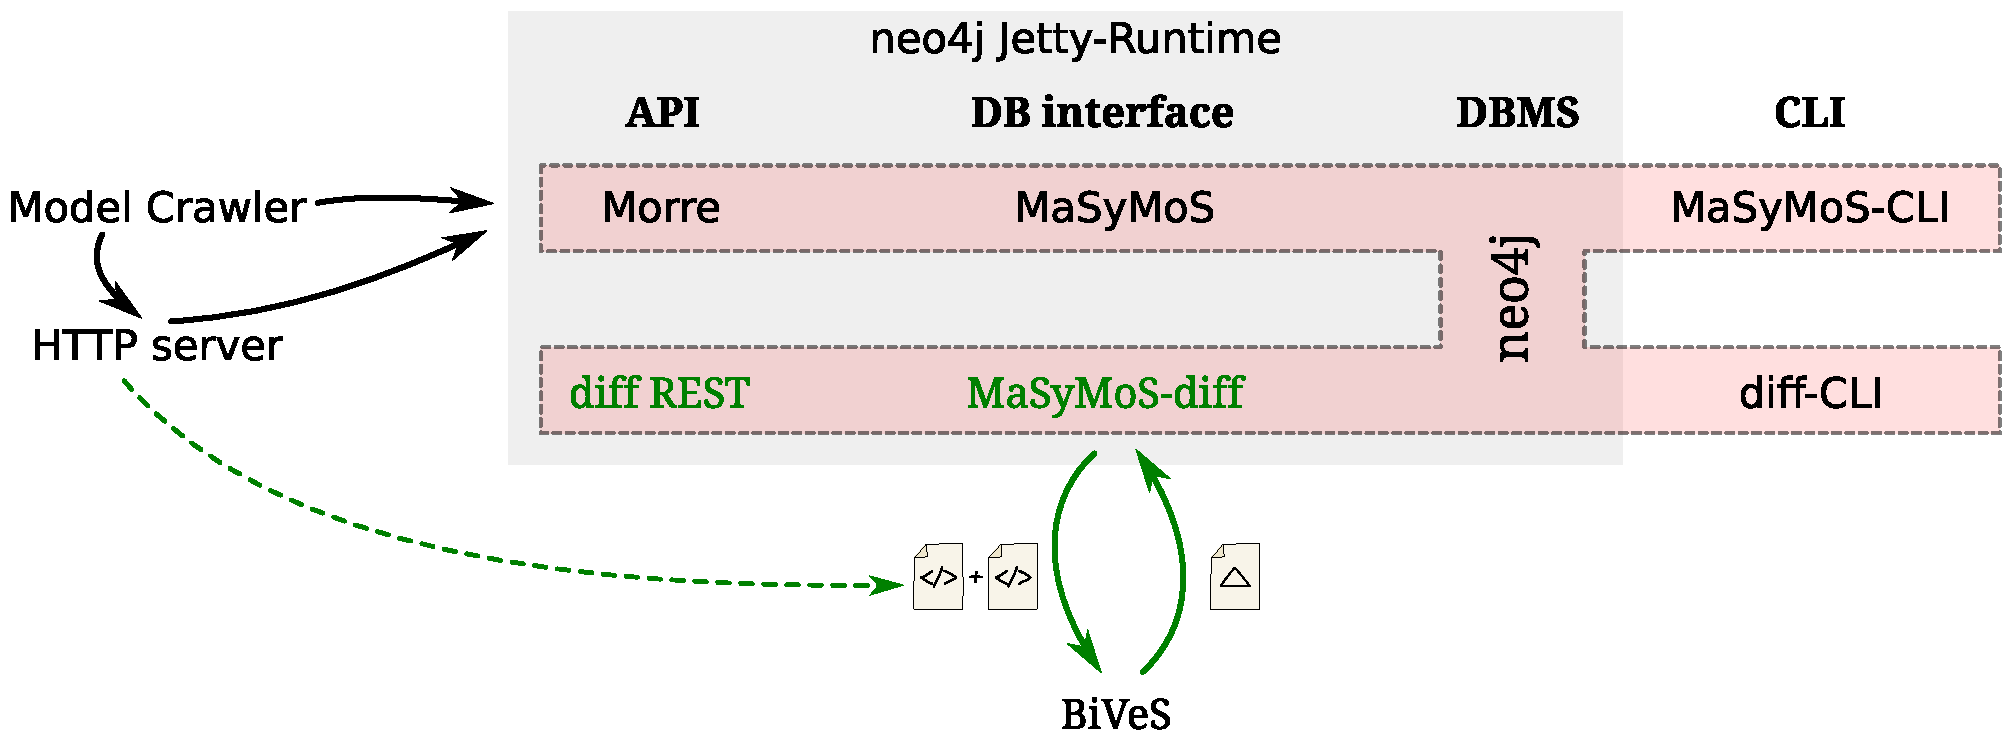
\includegraphics[width=\linewidth,height=\textheight,keepaspectratio]{../tex/resources/system-overview-matrix.pdf}
	\vfill
\end{frame}

\begin{comment}
\begin{frame}{Concept}{\neoj}
	{\Large \neoj}
	\\[2.5em]
	\begin{itemize}
		\item ...
	\end{itemize}
\end{frame}
\end{comment}

\begin{frame}{Concept}{\masymos data structure}
	\centering
	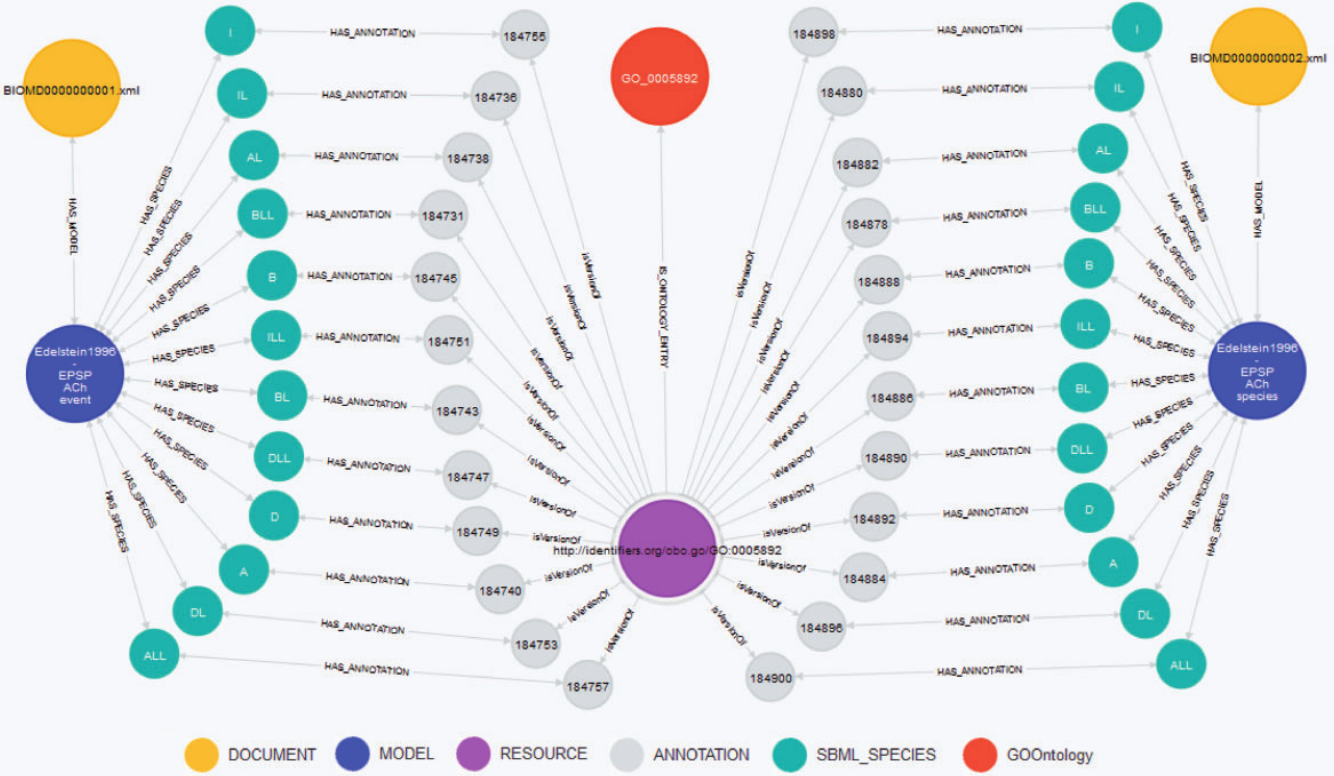
\includegraphics[width=\linewidth,height=\textheight,keepaspectratio]{./figures/masymos-small.png}\\
	{\small Figure taken from \citealt{Henkel2015}}
\end{frame}

\begin{frame}{Concept}{System Overview}
	{\LARGE System Overview}
	\\[2.5em]
	\centering
	\vfill
	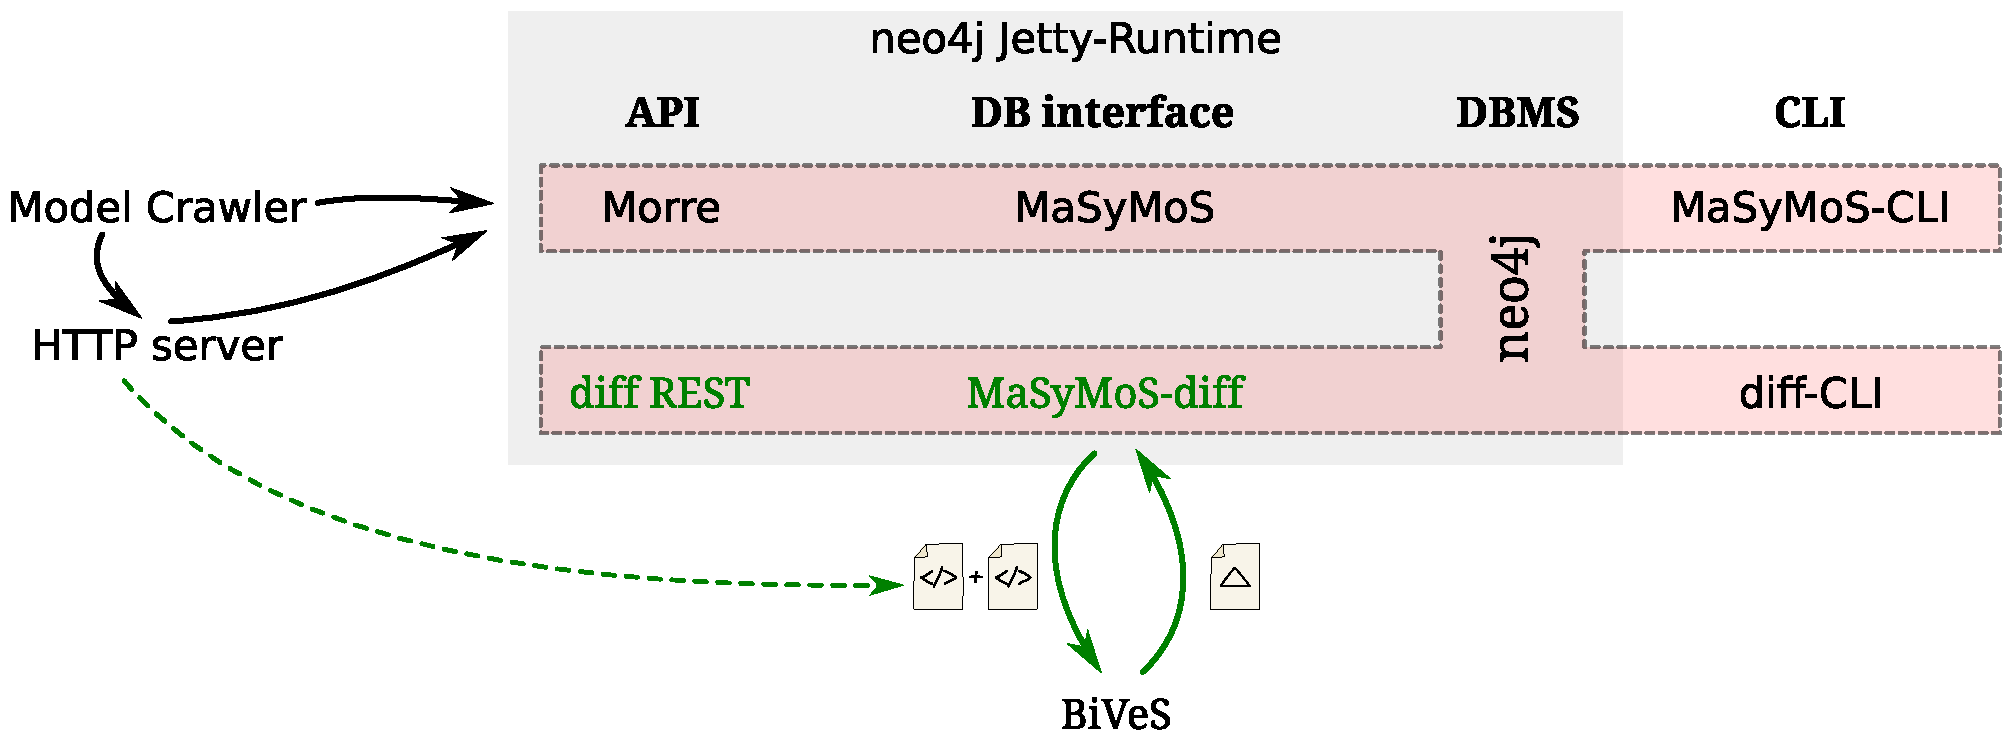
\includegraphics[width=\linewidth,height=\textheight,keepaspectratio]{../tex/resources/system-overview-matrix.pdf}
	\vfill
\end{frame}

\begin{frame}{Concept}{Database Extension}
	\centering
	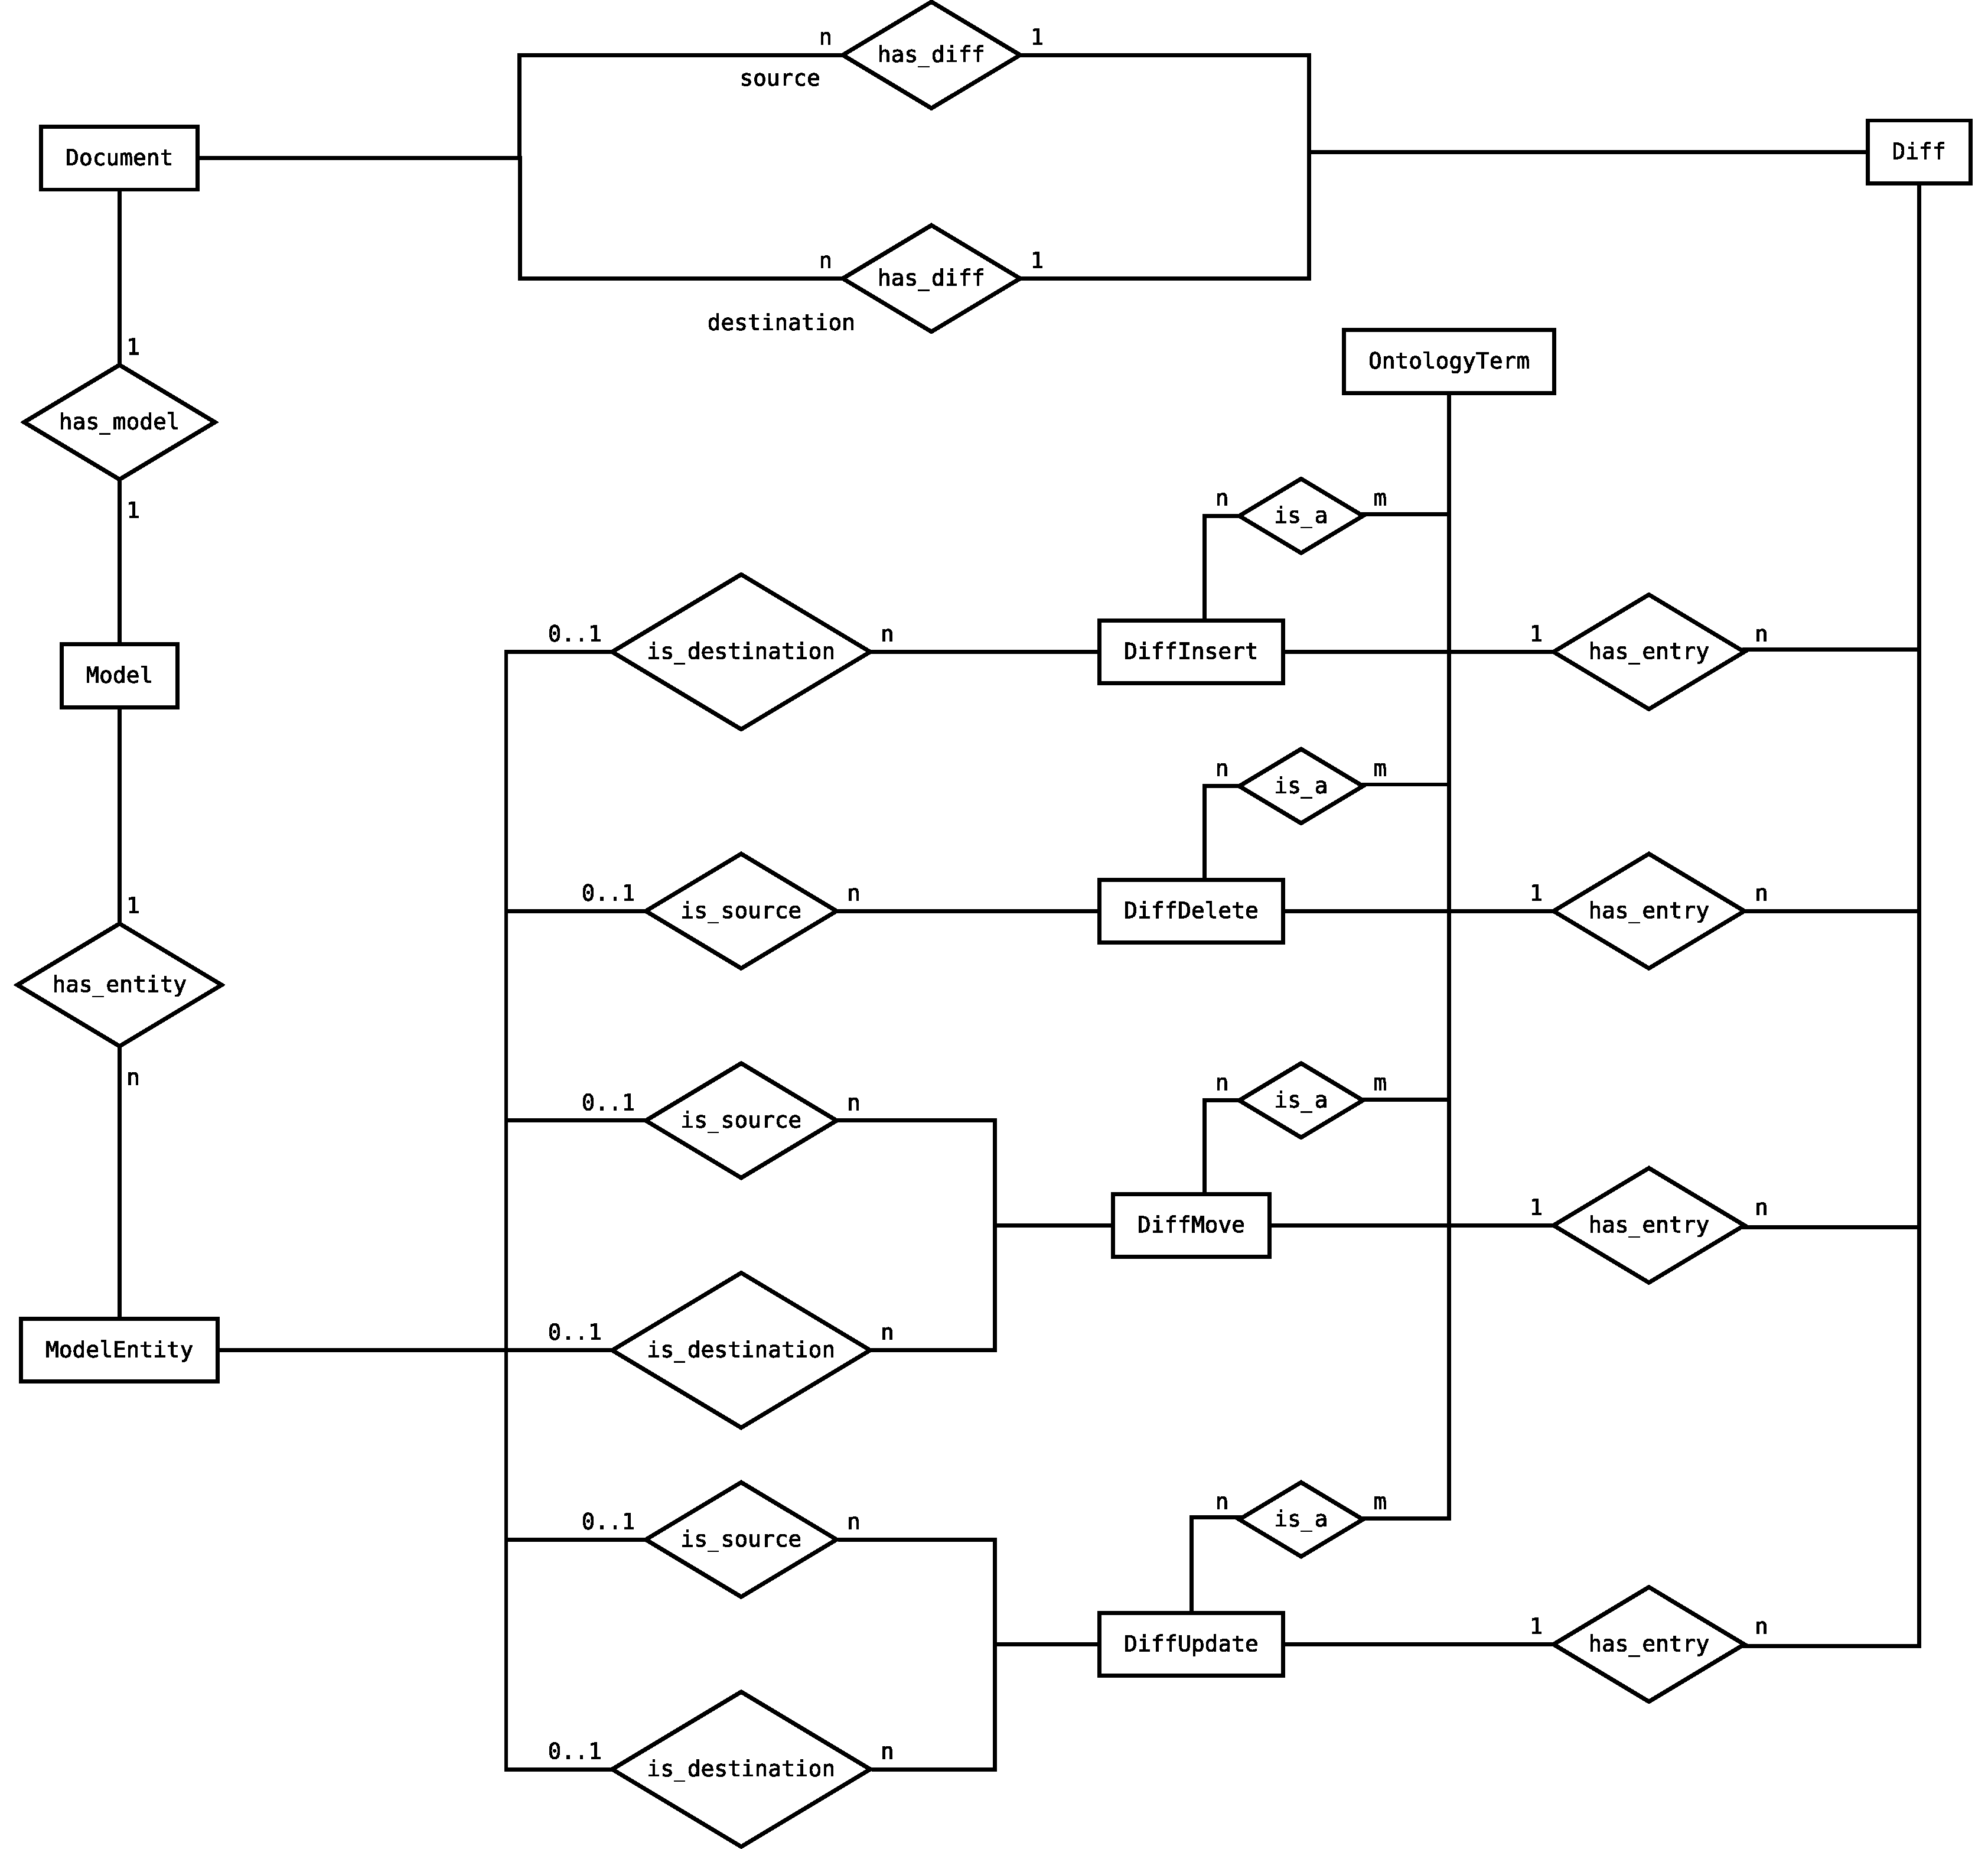
\includegraphics[width=\linewidth,height=\textheight,keepaspectratio]{../tex/resources/db-concept-er.pdf}
\end{frame}

\begin{frame}{Concept}{Database Extension}
	\centering
	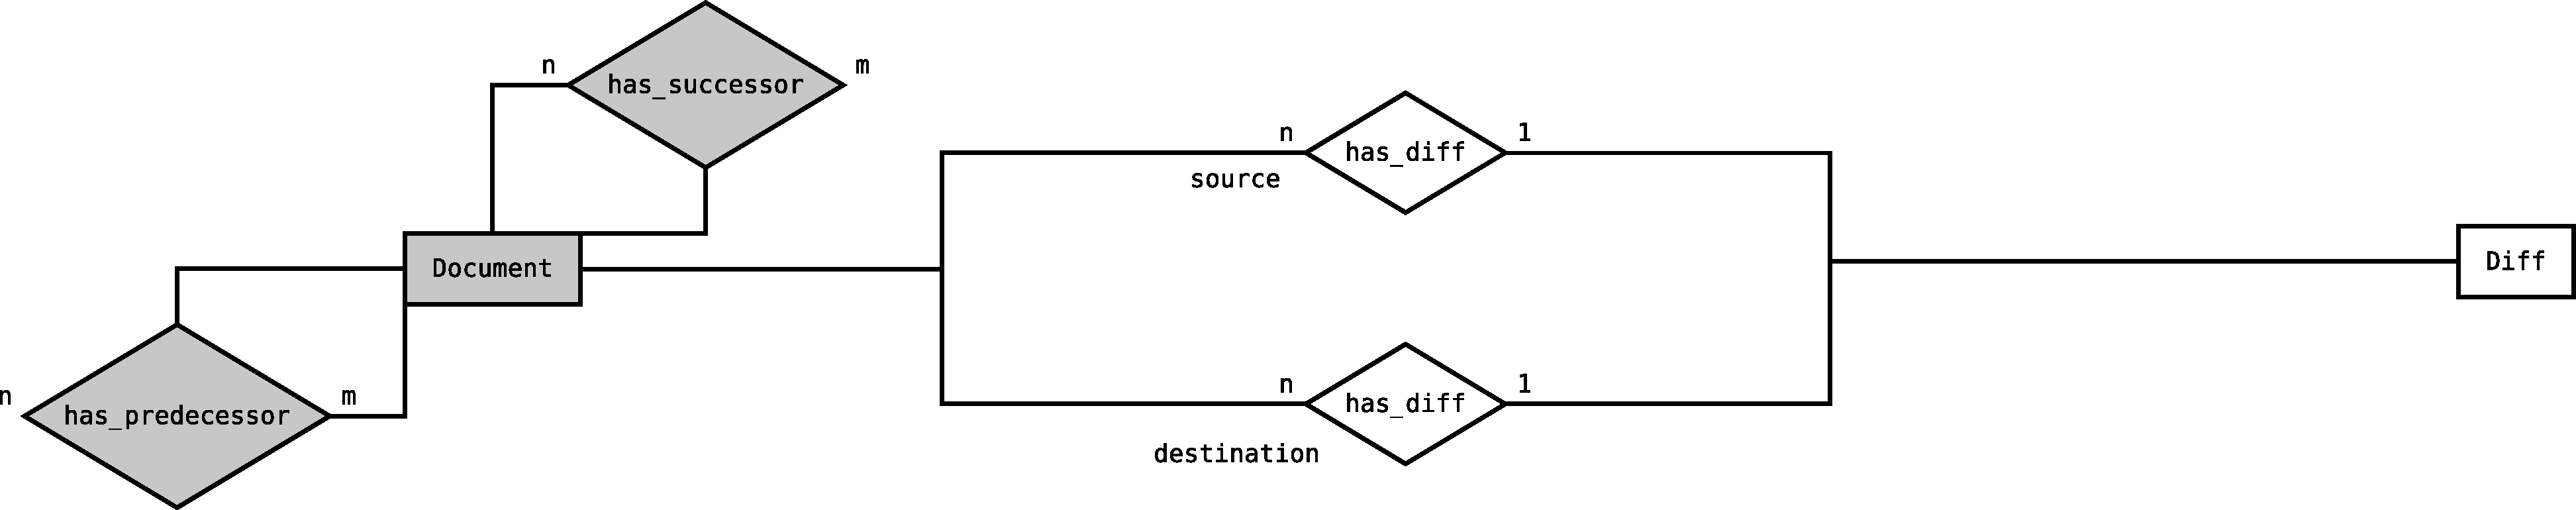
\includegraphics[width=\linewidth,height=\textheight,keepaspectratio]{figures/er-part-1.pdf}
\end{frame}

\begin{frame}{Concept}{Database Extension}
	\centering
	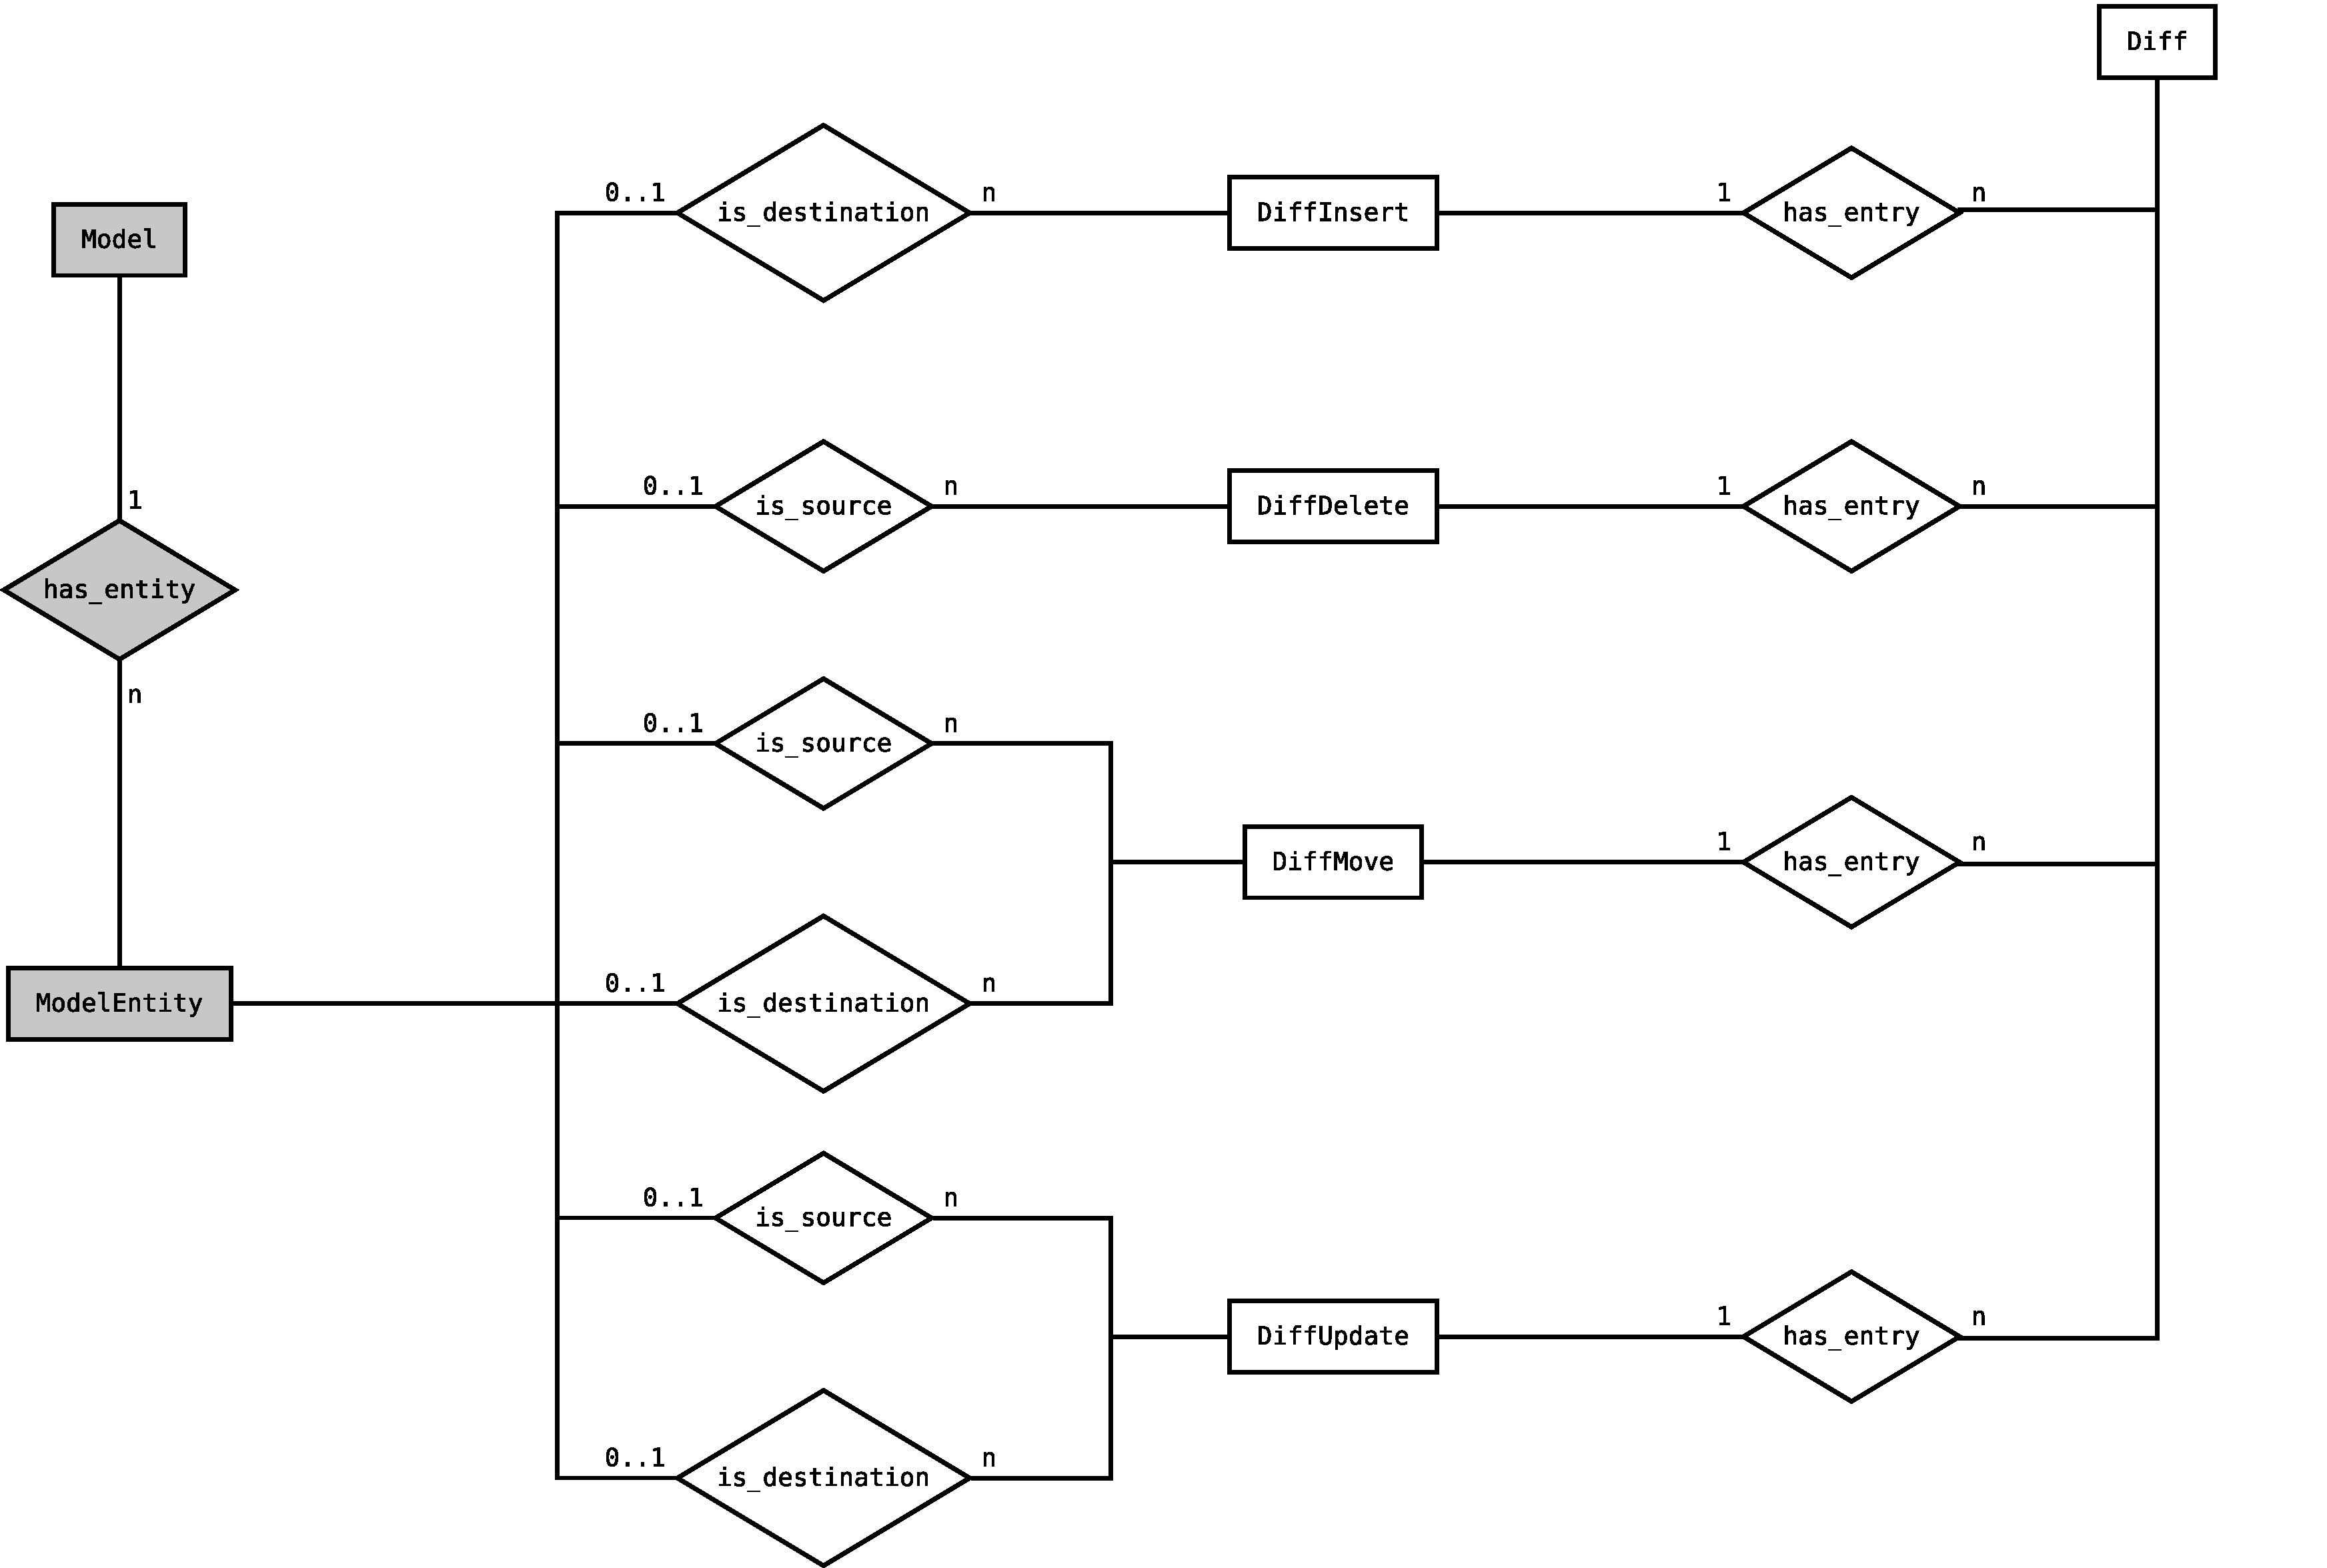
\includegraphics[width=\linewidth,height=\textheight,keepaspectratio]{figures/er-part-2.pdf}
\end{frame}

\begin{frame}{Concept}{Database Extension}
	\centering
	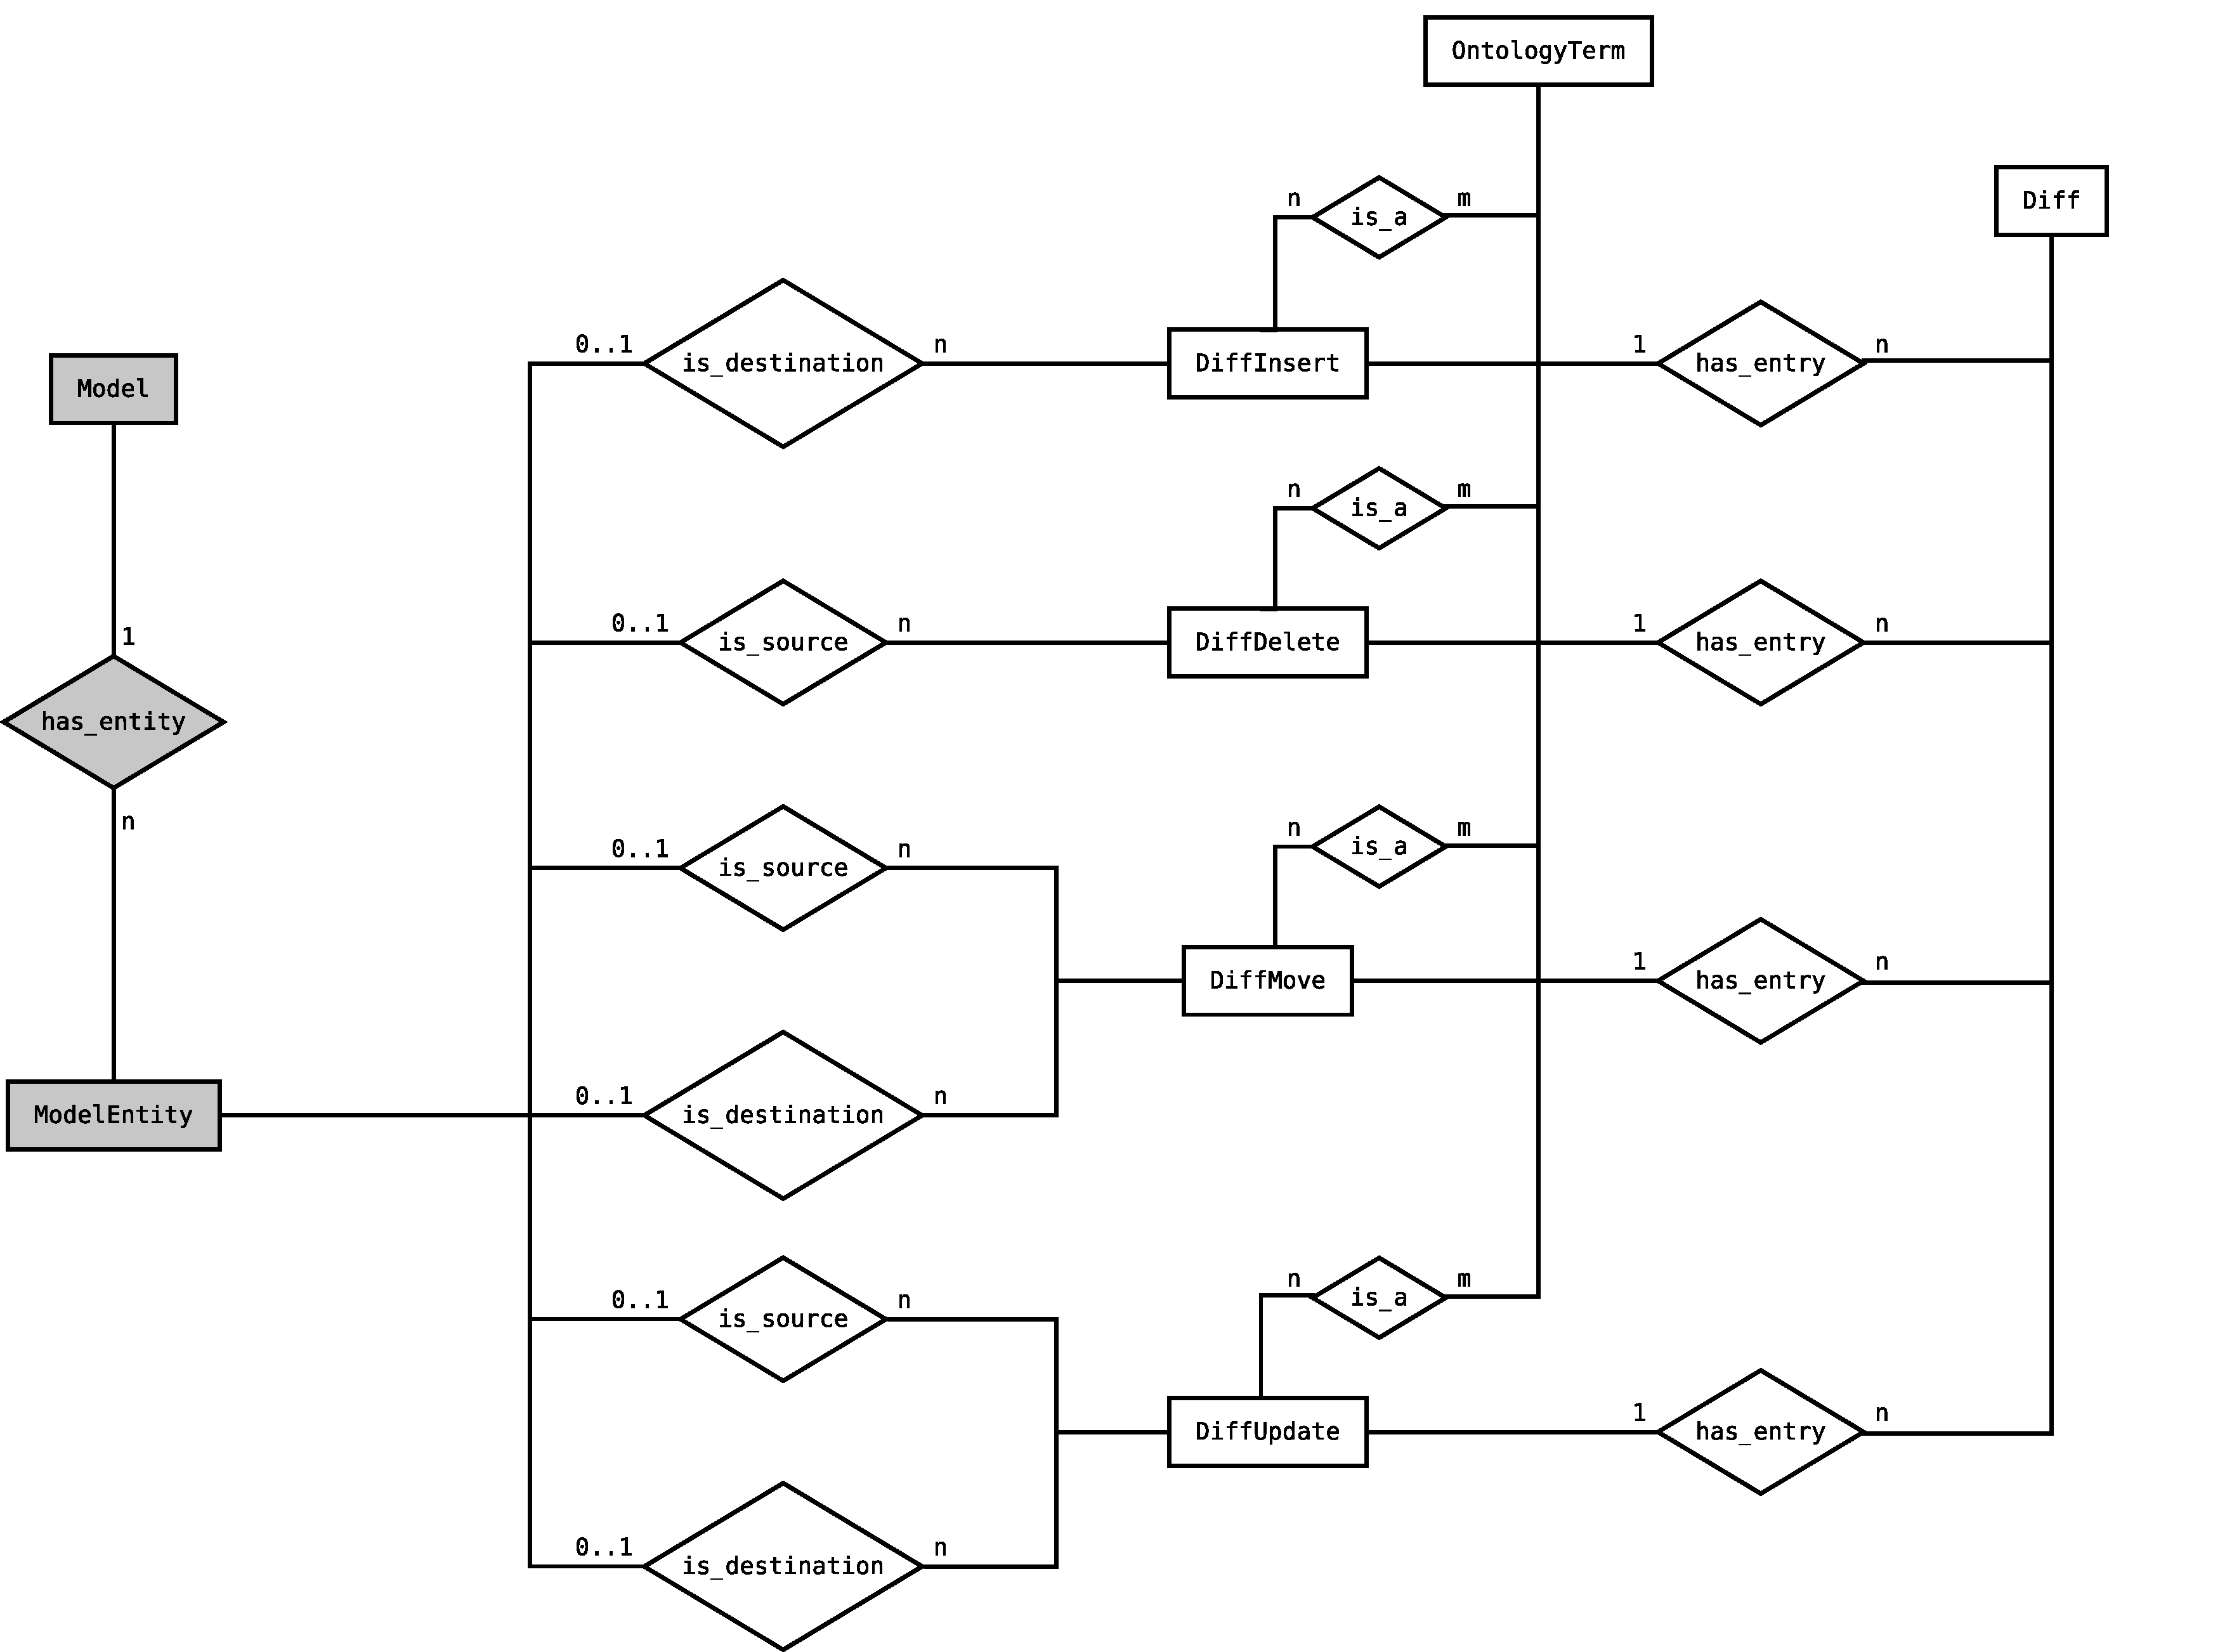
\includegraphics[width=\linewidth,height=\textheight,keepaspectratio]{figures/er-part-3.pdf}
\end{frame}

\begin{frame}{Concept}{Database Extension}
	\centering
	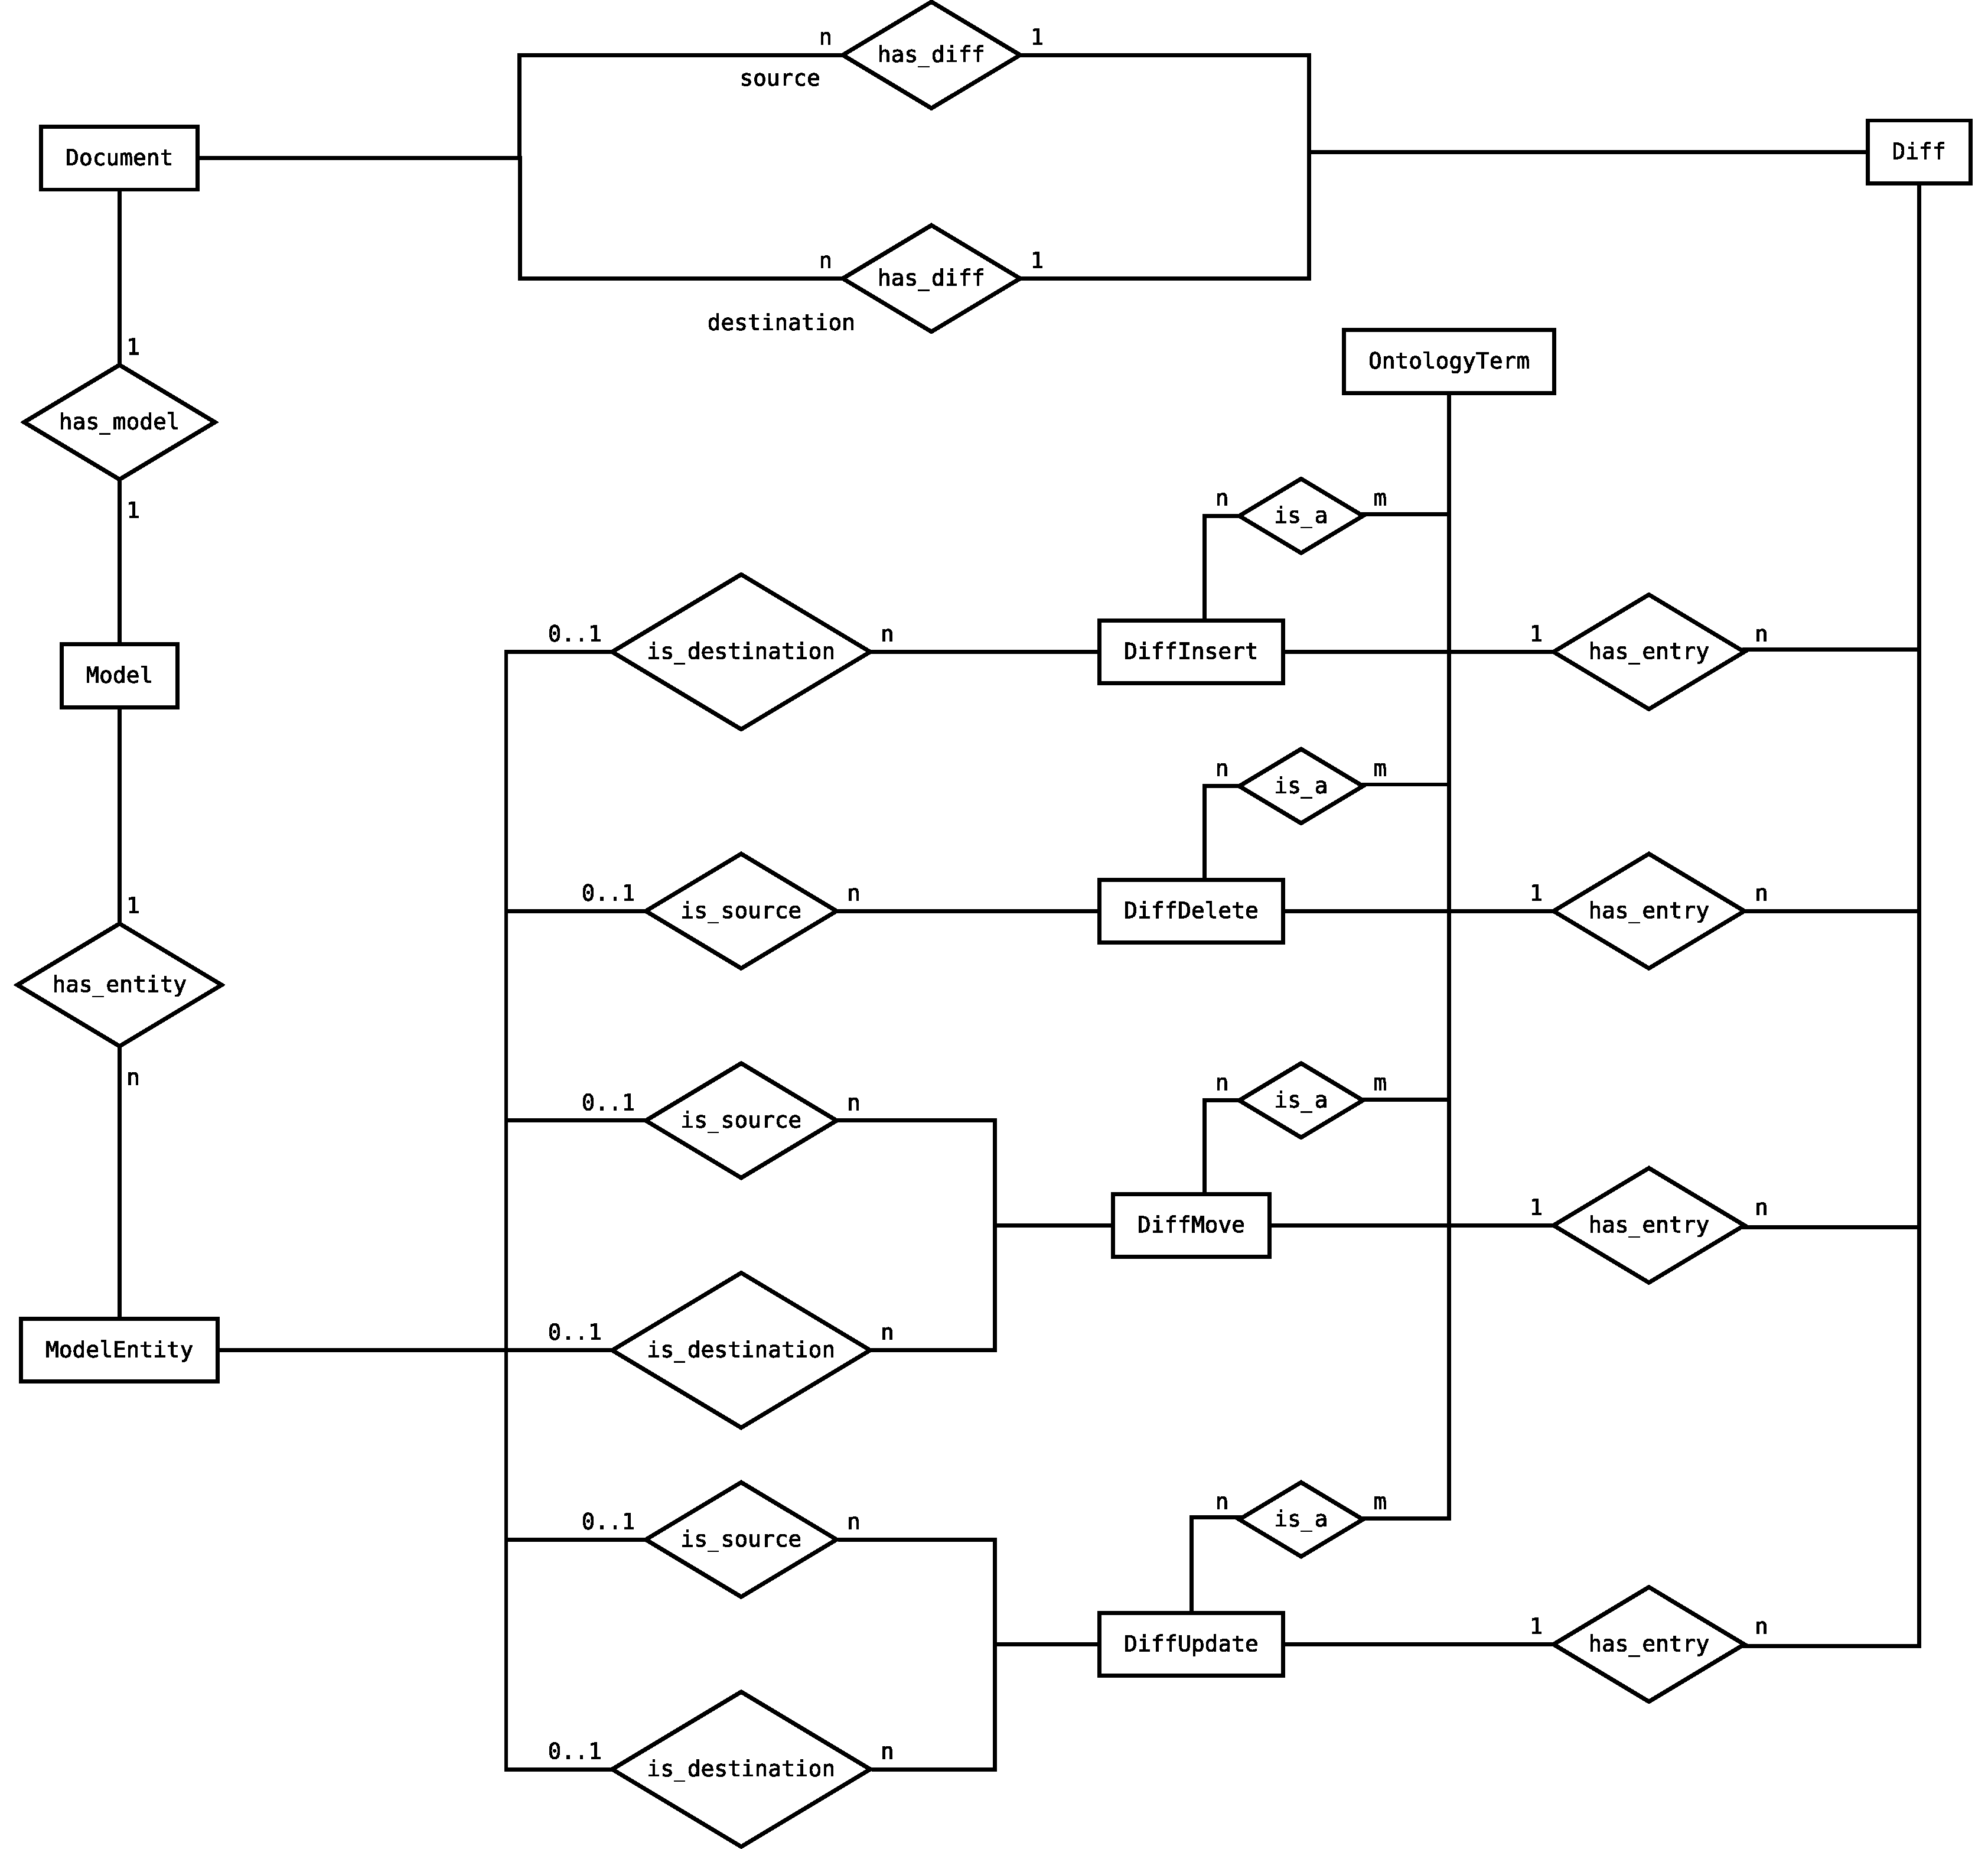
\includegraphics[width=\linewidth,height=\textheight,keepaspectratio]{../tex/resources/db-concept-er.pdf}
\end{frame}

\begin{frame}{Concept}{Database Extension}
	{\Large Database Extension as ER Model}
	\\[2.5em]
	\begin{itemize}
		\item Not storage efficient
		\item But easy to query
		\item Incorporation of semantic annotations with ontology terms
	\end{itemize}
\end{frame}

\newsection{Implementation}
\begin{frame}{Implementation}{}
	\centering
	\LARGE Implementation
\end{frame}

\begin{frame}{Implementation}{}
	{\Large Implementation Overview}
	\\[2.5em]
	\begin{itemize}
		\item \modelcrawler
		\item Extensions to the \masymos core
		\item Diff plugin
		\item \rest interface\\[2em]
		\item \textbf{Constraint:} Keep modifications to original \masymos code minimal.
	\end{itemize}
\end{frame}

\begin{frame}{Implementation}{\modelcrawler}
	{\Large The \modelcrawler}
	\\[2.5em]
	\begin{itemize}
		\item Java tool to crawl \emph{BioModels Database} and \emph{PMR2}
		\item Downloads and stores all model files
		\item Pushes new versions to \masymos
	\end{itemize}
\end{frame}

\begin{frame}{Implementation}{Extensions to the \masymos core}
	{\Large Extensions to the \masymos core}
	\\[2.5em]
	\begin{itemize}
		\item Importing ontologies with dynamic name\\
			$\rightarrow$ Hard coding names no longer required
		\item Implemented a \texttt{DynamicUniqueFactory}
		\item Ensures uniqueness for terms from ontologies with dynamic defined namespaces
	\end{itemize}
\end{frame}

\begin{frame}{Implementation}{Diff plugin}
	{\Large The diff plugin}
	\\[1.5em]
	\begin{itemize}
		\item Actual core of the delta/diff implementation\\
			$\rightarrow$ implemented as separate plugin, depending on \masymos
		\item Provides prioritized thread pool executor, for parallelization 
		\item Uses \bives library \citep{Scharm2015} to:
		\begin{itemize}
			\item Generate diffs of models with \comodi \citep{Scharm2016} annotations
			\item Parse model files, encoded in \sbml or \cellml
		\end{itemize}
		\item Inserts deltas into \neoj/\masymos
		\item Parses \xml/\rdf \comodi annotations and inserts them
	\end{itemize}
\end{frame}

\begin{frame}{Implementation}{A Database Dump}
	\centering
	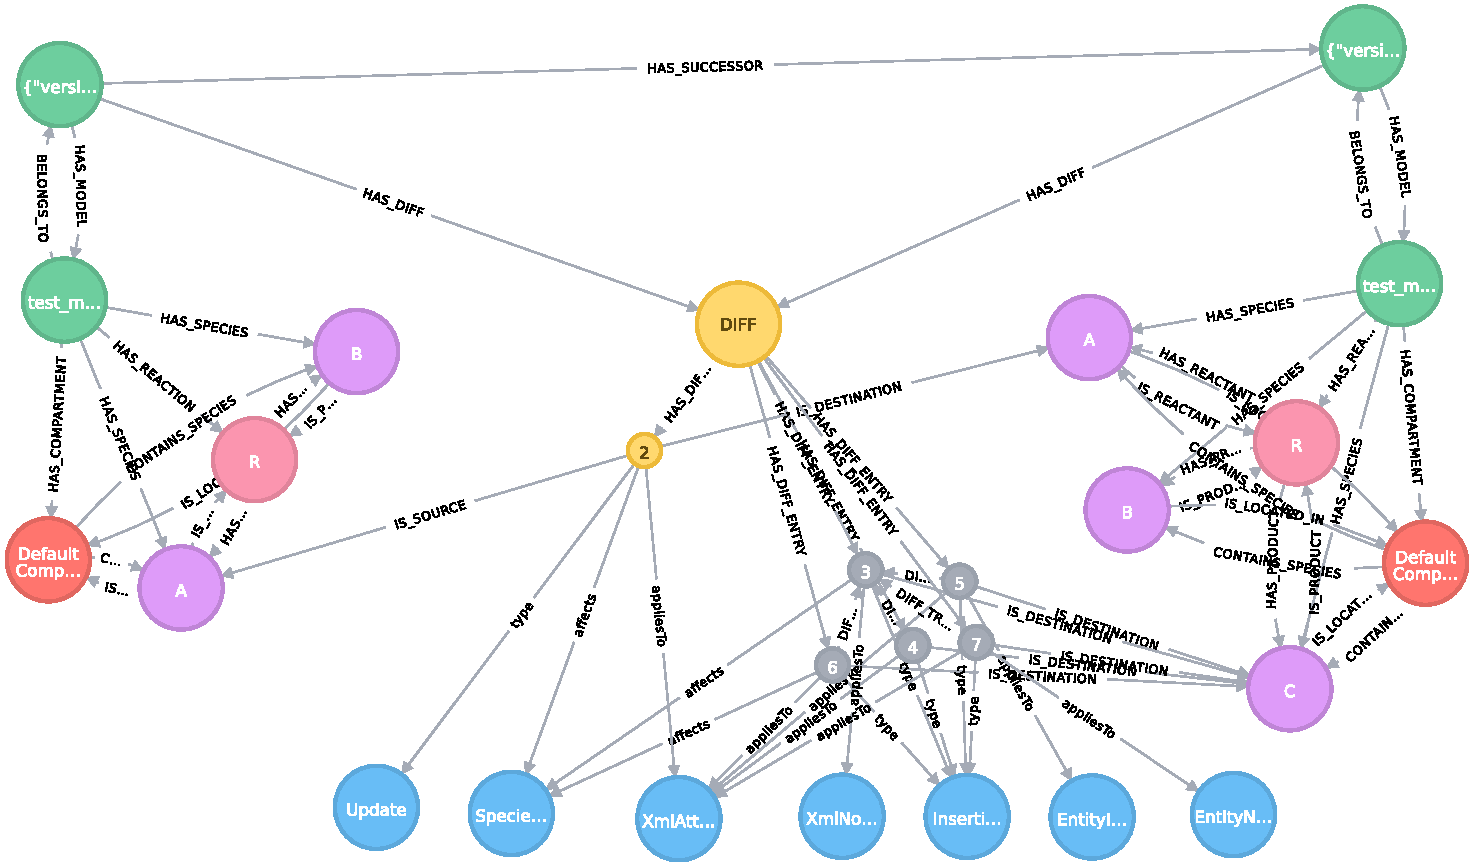
\includegraphics[width=\linewidth,height=\textheight,keepaspectratio]{../tex/resources/neo4j-renders/demo-sbml-simple-diff.pdf}
\end{frame}

\begin{frame}{Implementation}{\rest interface}
	{\Large \rest interface}
	\\[2.5em]
	\begin{itemize}
		\item \neoj unmanaged extension
		\item Providing \json/\rest interface using Jackson and JAX-RS
		\begin{itemize}
			\item Trigger Diff generation
			\item Check thread pool statistics
			\item Check database statistics
			\item Clean all diffs from the database
		\end{itemize}
	\end{itemize}
\end{frame}

\newsection{Outcome}
\begin{frame}{Outcome}{}
	\centering
	\LARGE Outcome
\end{frame}

\begin{frame}{Outcome}{}
	{\Large Outcome}
	\\[2.5em]
	\begin{itemize}
		\item A database concept to store multiple versions of biological models
		\begin{itemize}
			\item Easy to query
			\item Semantic annotations $\rightarrow$ allows to compare deltas on abstract layer
		\end{itemize}
		\item A Java implementation into existing infrastructure
		\begin{itemize}
			\item Extended \masymos to store differences between versions
			\item Parallelized thread pool executor to generate deltas
			\item \rest interface to monitor, trigger, and undo the diff generation
		\end{itemize}
	\end{itemize}
	
\end{frame}

\begin{frame}{Outcome}{Test Run}
	{\Large Test Run}
	\\[2.5em]
	\begin{itemize}
		\item Imported all models in \emph{BioModels Database} and \emph{PMR2} on 2016-10-14
		\item $3\,367$ distinct models
		\item $14\,503$ model versions
		\item $4.307$ versions per model on average
		\item $223\,144$ changes\\
			$128\,847$ inserts, $64\,457$ deletes, $15\,198$ updates, $14\,642$ moves
		\item $8.5$ GBytes of disc storage consumption for the database
	\end{itemize}
\end{frame}

\begin{frame}{Outcome}{Test Run Visualization}
	\centering
	\includegraphics[width=\linewidth,height=\textheight,keepaspectratio]{./figures/all-color-small.png}\\
	{\footnotesize Visualization of all 14 503 model versions and deltas between them}
\end{frame}

\begin{frame}{Scope of this Work}{What this work is not about}
	\centering
	
\includegraphics[width=\linewidth,height=\textheight,keepaspectratio]{./figures/xkcd-standards.png}\\
	{\small XKCD -- Standards \url{http://xkcd.com/927/}}
\end{frame}

\begin{frame}{It's done!}{}
	\centering
	\begin{tikzpicture}[>=stealth',trans/.style = {->,densely dashed,lightgray},shift={(0,0)},font=\small\selectfont]
	\node[anchor=center] (graph) at (0,0) {
		\includegraphics[width=\linewidth,height=\textheight,keepaspectratio]{./figures/all-color-small.png}
	};
	\node[anchor=center] (txt) at (graph.center) {
		\LARGE Thanks for your attention!
	};
	\end{tikzpicture}
\end{frame}
